\section{Privacy in Data Outsourcing}
L'avanzamento nell'ICT ha completamente cambiato la nostra società, le infrastrutture e i servizi sono molto più potenti, efficienti e complessi. Questo sviluppo nell'ICT ha aperto le porte per la creazione di una smart society. \\
Vantaggi degli smart devices:
\begin{itemize}
    \item migliori meccanismi di protezione
    \item business continuity e disaster recovery che mi danno la possibilità di continuare ad operare anche quando qualcosa va storto
    \item migliori capacità di prevedere e rispondere ad eventuali attacchi e intrusioni
\end{itemize}
D'altro canto però:
\begin{itemize}
    \item sistemi molto complessi dove il collegamento debole diventa un facile punto di attacco
    \item esplosione di danni e violazioni
    \item perdita del controllo di dati e processi (dove sono i miei dati e chi li gestisce?)
\end{itemize}
\begin{center}
    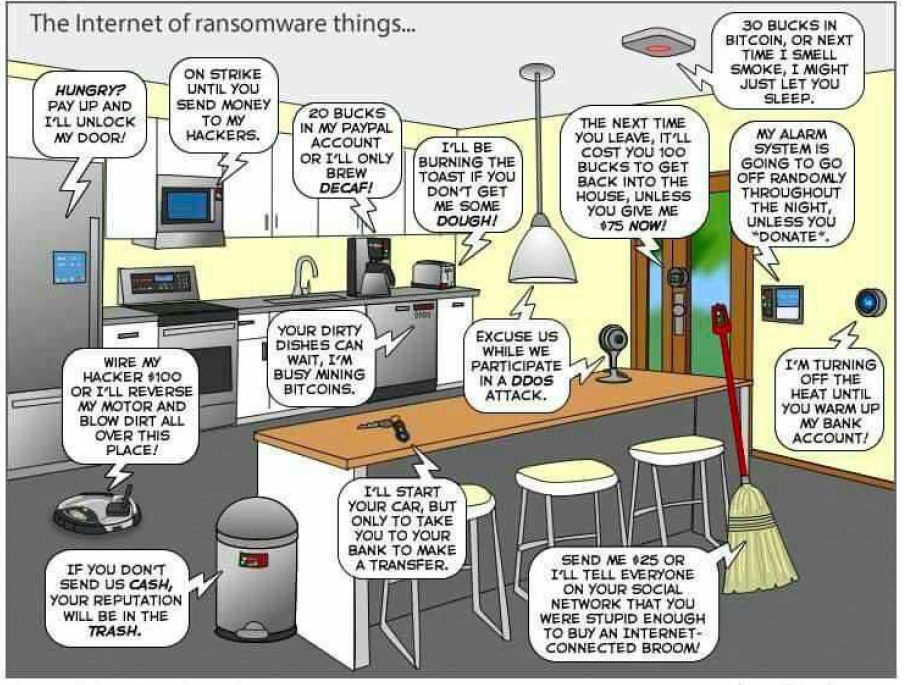
\includegraphics[scale=0.4]{img/com.png}
\end{center}
Diventa essenziale quindi chiedersi: cosa dobbiamo proteggere?
\begin{itemize}
    \item Infrastruttura
    \item Singole componenti
    \item Comunicazione
    \item Dati
\end{itemize}
Il ruolo dei dati in uno scenario smart è fondamentale:
\begin{center}
    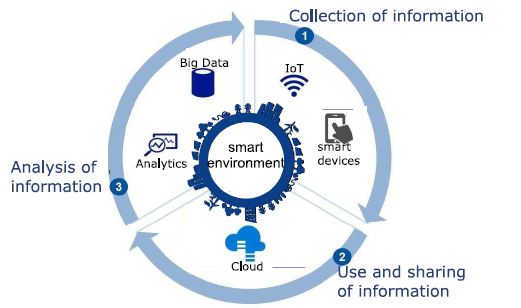
\includegraphics[scale=0.5]{img/smartenv.png}
\end{center}

\subsection{Cloud Computing}
Il cloud permette agli utenti e alle organizzazioni di affidarsi a provider esterni per immagazzinare, processare e accere ai loro dati, essenzialmente per: 
\begin{itemize}
    \item grandi possibilità di configurazione e scalabilità conveniente
    \item dati e servizi sempre accessibili
    \item infrastrutture scalabili per le applicazioni
\end{itemize}
Ma questo avviene tutto a discapito del controllo dei propri dati, introducendo così nuovi problemia livelli di sicurezza e privacy.\\
I Cloud Service Provider (CSPs) offrono una buona protezione, il problema è che questa protezione è relativa solo al perimetro del cloud provider. All’interno, se il provider ha la chiave può vedere i dati. \\
Perché al provider dovrebbe servire la chiave? Per dare servizi: se vuoi la risposta a una query, il provider deve poter leggere i dati. Questo implica una totale fiducia nel provider che ha completo accesso ai nostri dati (Google Drive, iCloud) \\
\begin{center}
    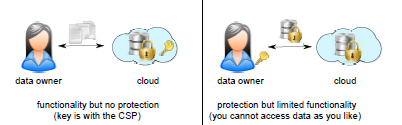
\includegraphics[scale=0.7]{img/csp.png}
\end{center}
Ci sono anche soluzioni dove il provider non possiede la chiave e questo rende molto oneroso riuscire fare delle query. Abbiamo quindi una protezione dei dati, ma limitate funzionalità siccome il CSP non può accedere ai dati (Boxcryptor, SpiderOak)\\
Negli ultimi tempi si stanno cercando delle soluzioni ibride dove si ha sia la protezione dei dati (rispetto all'esterno e rispetto al provider) che le funzionalità complete. In questo approccio vengono considerate sicure solo le operazioni dell'utente. 
\begin{center}
    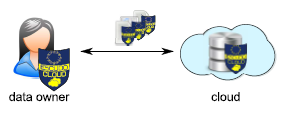
\includegraphics[scale=0.7]{img/escudo.png}
\end{center}
Quando si affronta la protezione dei dati bisogna cercare di \textbf{minimizzare} il rilascio e l'esposizione per evitare:
\begin{itemize}
    \item correlazione tra diverse sorgenti di dati
    \item inferenza indiretta usando dati esterni
\end{itemize}
\begin{center}
    \textbf{deidentificare} \( \neq \) \textbf{anonimizzare}
\end{center}

\subsection{Sfide nella Protezione dei Dati}
Queste sfide sono caratterizzate principalmente da tre dimensioni, riassunte nello schema seguente:
\begin{center}
    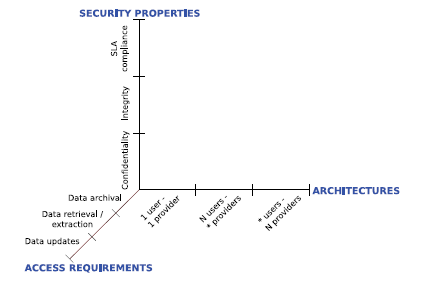
\includegraphics[scale=0.7]{img/secchall.png}
\end{center}
Nelle sezioni seguenti andremo ad analizzare una alla volta.

\subsubsection{Proprietà di Sicurezza}
\begin{itemize}
    \item \textbf{Confidenzialità}: mantenere la confidenzialità vuol dire permetterre l'accesso e la visione solo a chi è autorizzato e comprendono:
    \begin{itemize}
        \item dati che memorizzo all'esterno, sia rispetto al mondo esterno, sia rispetto al CSP
        \item identità degli utenti che utilizzano il sistema
        \item azioni che gli utenti fanno sui dati in quanto in alcuni casi non è confidenziale il dato in sè, ma lo è l'operazione che fa l'utente su di esso
    \end{itemize}
    \item \textbf{Integrità}: più complessa della confidenzialità perchè stiamo parlando di persone autorizzate che modificano i dati. Non è possibile sempre garantire l'integrità, possiamo invece fornire una specie di backup che mi garantisce "l'integrità" (capisco se i dati sono stati compromessi e li recupero con la tecnica di ridondanza degli stessi). Questa deve essere garantita:
    \begin{itemize}
        \item rispetto ai dati che ho memorizzato all'esterno
        \item rispetto ai risultati delle computazioni e delle query (più complicato perchè effettuato dinamicamente)
    \end{itemize}
    \item \textbf{Conformità al Service Level Agreement (SLA)}: garantire conformità rispetto allo SLA che si è sottoscritto, il che comprende:
    \begin{itemize}
        \item garanzia e certificati
        \item disponibilità
    \end{itemize}
\end{itemize}

\subsubsection{Requisiti di Accesso}
\begin{itemize}
    \item \textbf{Archiviazione dei dati}: semplice archiviazione dei dati
    \begin{itemize}
        \item upload e download
        \item solo protezione dei dati
    \end{itemize}
    \item \textbf{Estrazione e Retrieve dei Dati}: 
    \begin{itemize}
        \item query selettive, dove il provider entra nei dati, li legge e mi fornisce il risultato della query
        \item protezione sulla computazione delle query (potrebbero essere confidenziali e il CSP non dovrebbe essere in grado di conoscere)
    \end{itemize}
    \item \textbf{Aggiornamento dei Dati}: dati dinamici che possono cambiare
    \begin{itemize}
        \item supporto all'accesso e all'aggiornamento dei dati
        \item protezione della privacy delle operazioni sui dati
    \end{itemize}
\end{itemize}

\subsubsection{Architetture}
\begin{itemize}
    \item \textbf{1 user - 1 provider}
    \begin{itemize}
        \item protezione dei dati in storage
        \item query specifiche
        \item privacy nelle query e nell'integrità dei dati
    \end{itemize}
    \item \textbf{n users - * providers}: 
    \begin{itemize}
        \item controllo delle autorizzazioni e degli accessi
        \item più scrittori
    \end{itemize}
    \item \textbf{* users - n providers}:
    \begin{itemize}
        \item controllo e regolazione dello scambio dei dati tra più providers
    \end{itemize}
\end{itemize}

\subsubsection{Combinazioni delle dimensioni}
Ogni combinazione delle istanze delle dimensioni identifica nuovi problemi e nuove sfide. Le proprietà di sicurezza che devono essere garantite dipendono dai requisiti di accesso e dall'assunzione di fiducia nel provider coinvolto.\\
I provider possono essere:
\begin{itemize}
    \item curiosi
    \item prigri
    \item maliziosi
\end{itemize}

\subsubsection{Problemi da affrontare}
\begin{itemize}
    \item privacy degli utenti
    \item protezione dei dati
    \item esecuzione delle query
    \item accessi privati
    \item controlli di accesso
    \item integrità e correttezza dei dati
    \item pubblicazione dei dati
    \item esecuzione di query collaborative
\end{itemize}

